\section{Boolsche Algebra}
\subsection{Rechenregel}
Alternative Schreibweisen:
$\overline{x} = \lnot x = NOT \quad + = V = OR \quad * = \Lambda = AND \quad  \text{\$ } = \oplus = XOR$

\begin{minipage}{0.11\textwidth}
	\begin{align*}
		a + 0 &= a \\
		a * 0 &= a \\
		a \text{ \$ } 0 &= a
	\end{align*}
\end{minipage}
\begin{minipage}{0.11\textwidth}
	\begin{align*}
		a + 1 &= 1 \\
		a * 1 &= a\\
		a \text{ \$ } 1 &= \overline{a}
	\end{align*}
\end{minipage}
\begin{minipage}{0.11\textwidth}
	\begin{align*}
		a + a &= a \\
		a * a &= a \\
		a \text{ \$ } a &= 0
	\end{align*}
\end{minipage}
\begin{minipage}{0.11\textwidth}
	\begin{align*}
		a + \overline{a} &= 1 \\
		a * \overline{a} &= 0 \\
		a \text{ \$ } \overline{a} &= 1
	\end{align*}
\end{minipage}

\begin{minipage}{0.2\textwidth}
	\begin{align*}
		a + b &= b + a \\
		a * b &= b * a \\
		a \text{ \$ } b &= b \text{ \$ } a
	\end{align*}
\end{minipage}
\begin{minipage}{0.2\textwidth}
	\begin{align*}
		(a + b) + c &= a *(b + c) \\
		(a * b) * c &= a *(b * c) \\
		(a \text{ \$ } b) \text{ \$ } c &= a \text{ \$ }(b \text{ \$ } c)
	\end{align*}
\end{minipage}

\begin{minipage}{0.2\textwidth}
	\begin{align*}
		a * (b + c) &= (a * b) + (a * c) \\
		a + (b * c) &= (a + b) * (a + c) \\
		a * (b \text{ \$ } c) &= (a * b) \text{ \$ } (a * c) \\
		a \text{ \$ } b &= (\overline{a} * b) + (a * \overline{b})
	\end{align*}
\end{minipage}
\begin{minipage}{0.2\textwidth}
	\begin{align*}
		a + (a * b) &= a \\
		a * (a + b) &= a \\
		(a + \bar{b}) * b &= a * b \\
		(a * \bar{b}) + b &= a + b \\
		(a * \bar{b}) \text{ \$ } b &= a + b \\
		(a \text{ \$ } \overline{b}) * b &= a * b	
	\end{align*}
\end{minipage}

\begin{minipage}{0.2\textwidth}
	\begin{align*}
		(a * b) + (a * \overline{b}) &= a \\
		(a + b) * (a + \overline{b}) &= a
	\end{align*}
\end{minipage}
\begin{minipage}{0.2\textwidth}
	\begin{align*}
		\overline{(a + b)} &=  \overline{a} * \overline{b} \\
		\overline{(a * b)} &=  \overline{a} + \overline{b}
	\end{align*}
\end{minipage}

\subsection{Inversionsgesetze}
\noindent \textbf{DeMorgan}: Alle Eingänge und Ausgänge von allen Gattern invertiert, sowie AND zu OR Gatter tauschen $\rightarrow$ Man erhält \underline{das selbe} Verhalten. \\
\noindent \textbf{Shanon}: Alle Haupteingänge invertiert, und AND zu OR und umgekehrt $\rightarrow$ Man erhält die \underline{invertierte} Schaltung.

\subsection{Kanonische Normalformen}
\noindent\begin{minipage}{\textwidth}
	KV-Diagramm Vorlagen\\
	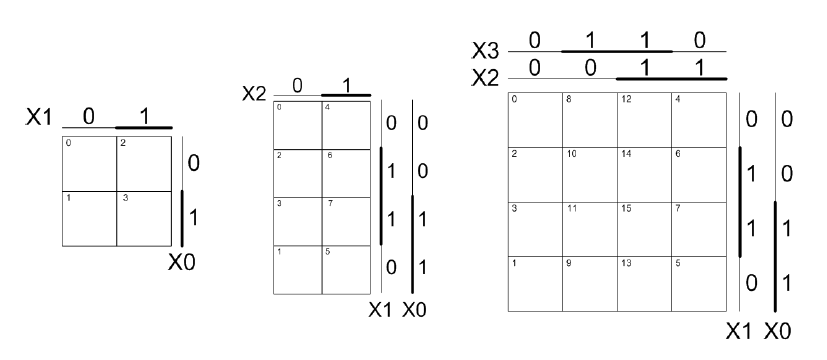
\includegraphics[height=11em]{./Images/DNF-3i-Diagram.png}
\end{minipage}

\noindent\begin{minipage}{\textwidth}
	\textbf{KKNF} - Kanonische konjunktive Normalform - \textbf{Nur 0}\\
	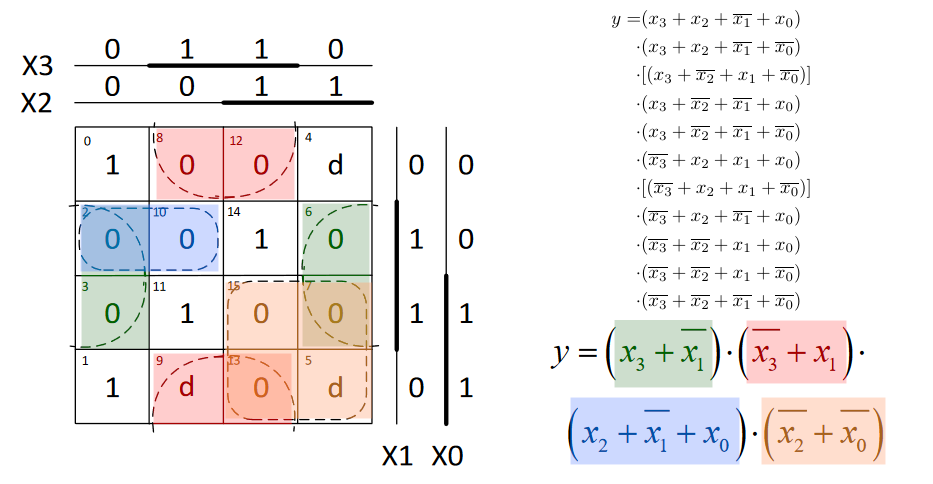
\includegraphics[height=11em]{./Images/KNF-Diagram.png}
\end{minipage}

\noindent\begin{minipage}{\textwidth}
	\textbf{KDNF} - Kanonische disjunktive Normalform - \textbf{Nur 1}\\
	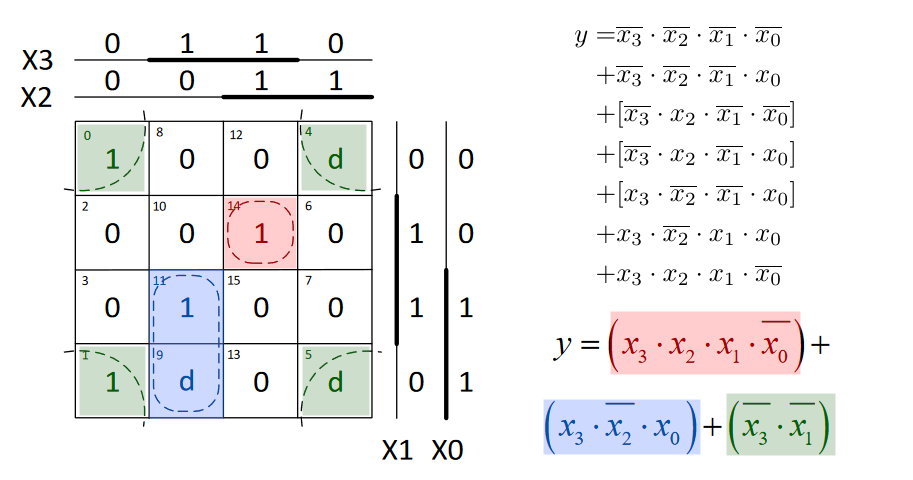
\includegraphics[height=11em]{./Images/DNF-Diagram.png}
\end{minipage}

